\documentclass{letask}

\begin{document}
\begin{titlepage}
\center % Center everything on the page
 
%----------------------------------------------------------------------------------------
%	HEADING SECTIONS
%----------------------------------------------------------------------------------------

\textsc{\LARGE Московский\\[-0.2cm]Физико-Технический Институт\\[0.1cm]\large (государственный университет)}\\[1.5cm] % Name of your university/college
\textsc{\Large Кафедра общей физики}\\[0.1cm] % Major heading such as course name
\textsc{\large Лабораторная работа \textnumero  4.4.1}\\[0.5cm] % Minor heading such as course title

%----------------------------------------------------------------------------------------
%	TITLE SECTION
%----------------------------------------------------------------------------------------

\HRule
\\[0.4cm]
{ \huge \bfseries Амплитудная\\[0.2cm]
дифракционная решетка}
\\[0.6cm] % Title of your document
\HRule
\\[1.5cm]


 
%----------------------------------------------------------------------------------------
%	AUTHOR SECTION
%----------------------------------------------------------------------------------------

\begin{minipage}{0.4\textwidth}
	\begin{flushleft} \large
		\textsf{Студент}
		
		Ришат \textsc{Исхаков} \\[-0.15cm]
		513 группа
	\end{flushleft}
\end{minipage}
~
\begin{minipage}{0.4\textwidth}
	\begin{flushright} \large
		\textsf{Преподаватель}
		
		Александр Александрович \\[-0.15cm]
		\textsc{Казимиров} % Supervisor's Name
	\end{flushright}
\end{minipage}

\begin{bottompar}
	\begin{center}
		
\includegraphics[width = 80 mm]{logo.jpg}
	\end{center}
	{\large \today}

\end{bottompar}
\vfill % Fill the rest of the page with whitespace

\end{titlepage}

\textbf{Цель работы:} знакомство с работой и настройкой гониометра Г5, определение спектральных характеристик амплитудной решетки.

\textbf{В работе используются:} гониометр, дифракционная решетка, ртутная лампа.

\section{Теоретическая часть}

Амплитудную решетку можно представить в виде непрозрачного экрана, в котором прорезано большое число $N$ параллельных щелей - штрихов, расстояние между которыми $d$ (шаг решетки).


Пусть на решетку падает излучение с длиной волны $\lambda$ по нормали к плоскости решетки. Вследствие дифракции лучи, прошедшие через щель в решетке, отклоняются от своего первоначального направления. Рассмотрим лучи, отклонившиеся на угол $\varphi$. Разность хода лучей о эквивалентных точек двух соседних штрихов равна 
\[ \Delta = d \sin \varphi .\]

Если эта величина равна целому числу длин волны:
\[ d \sin \varphi = m \lambda, \quad m = 0, \pm 1, \pm 2, ... ,\]
то волны взаимно усиливают друг друга.


В соответствии с принципом Гюйгенса–Френеля распределение интенсивности в дифракционной картине определяется суперпозицией волн, приходящих в точку наблюдения от различных щелей решётки. При этом амплитуды всех интерферирующих волн при заданном угле $\varphi$ практически одинаковы, а фазы составляют арифметическую прогрессию.


\[
I = I_0 \dfrac{sin^2[N(kd \sin{\varphi})/2]}{sin^2[(kd \sin{\varphi})/2]},
\]

где $k$~--~волновое число, $I_0$~--~интенсивность волны, идущей от одного штриха. При большом числе щелей свет, прошедший через решётку, распространяется по ряду резко ограниченных направлений. Если на дифракционную решётку падает свет сложного спектрального состава, то после решётки образуется спектр, причём фиолетовые лучи отклоняются решёткой меньше, чем красные (чем больше длина волны, тем сильнее лучи отклоняются решеткой). Входящая в величина $m$ носит название порядка спектра. При $m = 0$ максимумы интенсивности для всех длин волн располагаются при $\varphi = 0$ и накладываются друг на друга. При освещении белым светом нулевой максимум, в отличие от всех прочих, оказывается поэтому неокрашенным. Спектры первого, второго и т.д. порядков располагаются симметрично по обе стороны от нулевого.



\textbf{Угловая дисперсия} $D$ характеризует угловое расстояние $d \varphi$ между спектральными линиями, отстоящими по длине волны на $d \lambda$:
\[
D=\dfrac{d \varphi}{d \lambda}=\frac{m}{d cos \varphi}=\dfrac{m}{\sqrt{d^{2}-(m \lambda)^{2}}}
\]

\textbf{Разрешающая способность дифракционной решетки.} Возможность разрешения двух близких спектральных линий зависит от их ширины и от расстояния между ними. Угловое расстояние между двумя близкими спектральными компонентами с длинами волн $\lambda$ и ($\lambda + \Delta \lambda$) равно:
\[
\Delta \varphi =  D d \lambda = \frac{m \Delta \lambda}{d \cos{\varphi}}.
\]

Согласно критерию Рэлея линии становятся неразличимыми, когда расстояние между ними меньше, чем расстояние от максимума одной линии до её первого минимума. Пусть решетка имеет $N$ штрихов. Выберем главный максимум $m$-го порядка для компоненты $\lambda$. Направление на первый дифракционный минимум дается равенством 
\[ d \sin \varphi = \left( m + \dfrac{1}{N} \right) \lambda. \]
По критерию Рэлея это же направление должно соответствовать главному дифракционному максимуму для второй компоненты $\lambda + \Delta \lambda$:
\[ d \sin \varphi = m (\lambda + \Delta \lambda) .\]
Из последних двух равенств находим 
\[\Delta \lambda = \dfrac{\lambda}{mN}.\]
По определению разрешающая способность спектрального прибора $R = \lambda / \Delta \lambda$~--~это отношение длины волны к разности длин волн двух линий, разрешаемых по критерию Рэлея.

Таким образом, приходим к следующему выражению для разрешающей способности дифракционной решетки:
\[R = \lambda / \Delta \lambda = mN\]

\section{Установка для измерений}

\begin{figure}[H]
\centering
	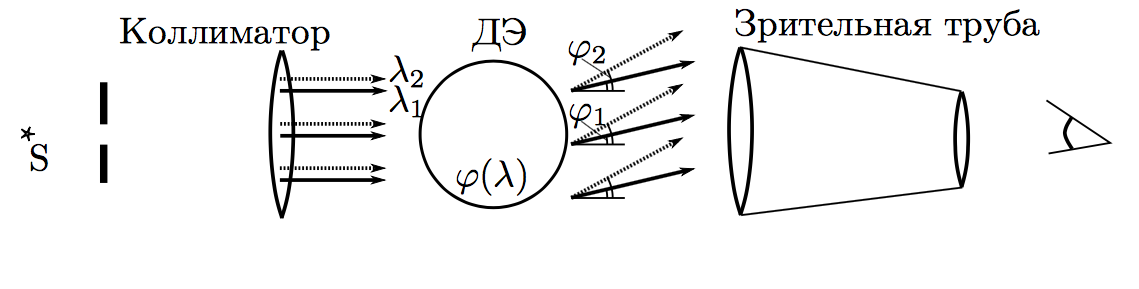
\includegraphics[width = \lw]{scheme}
	\caption{Схема прибора: источник-коллиматор -- диспергирующий элемент -- зрительная труба}
	\label{fig:scheme}
\end{figure}

Исследование спектра ртутной лампы, определение периода и спектральных характеристик решетки проводится с помощью гониометра Г5.

\begin{figure}[H]
\centering
	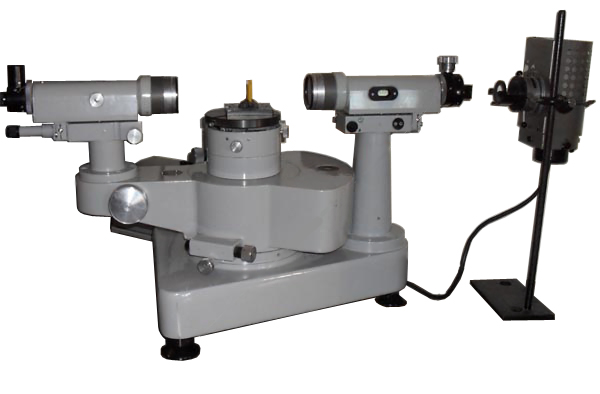
\includegraphics[width = 0.7\lw]{g5}
	\caption{Внешний вид гониометра Г5}
	\label{fig:g5}
\end{figure}


\section{Измерения}
\begin{enumerate}
  \item Подберем ширину входной щели коллиматора так, чтобы ширина линий жёлтого дублета была чуть больше промежутка между линиями двойного штриха окуляра зрительной трубы. Установим высоту щели, удобную для измерений.
\[\delta \varphi = \ang{;;5}\]
\begin{table}[H]
\centering
\caption{Измерим угловые координаты спектральных линий ртути для $\pm 1$ порядка}
\begin{tabular}{|c|c|c|c|c|c|}
\hline
Порядок & Цвет & $\lambda$   & $\varphi$   & $\sin \varphi $  & $\delta (\sin \varphi)$\\ \hline
1       & Фиолетовый & 404.7 & \ang{168;22;18} & 0.202  & 0.0012 \\ \hline
1       & Синий      & 435.8 & \ang{167;26;54} & 0.217  & 0.0013 \\ \hline
1       & Голубой    & 491.6 & \ang{165;48;54} & 0.245  & 0.0015 \\ \hline
1       & Зеленый    & 546.1 & \ang{164;12;08} & 0.272  & 0.0016 \\ \hline
1       & Желтый 1   & 577   & \ang{163;16;22} & 0.288  & 0.0017 \\ \hline
1       & Желтый 2   & 579.1 & \ang{163;12;12} & 0.289  & 0.0018 \\ \hline
-1      & Фиолетовый & 404.7 & \ang{191;40;32} & -0.202 & 0.0012 \\ \hline
-1      & Синий      & 435.8 & \ang{192;32;32} & -0.217 & 0.0013 \\ \hline
-1      & Голубой    & 491.6 & \ang{194;12;58} & -0.246 & 0.0015 \\ \hline
-1      & Зеленый    & 546.1 & \ang{195;50;50} & -0.273 & 0.0017 \\ \hline
-1      & Желтый 1   & 577   & \ang{196;45;09} & -0.288 & 0.0017 \\ \hline
-1      & Желтый 2   & 579.1 & \ang{196;48;55} & -0.289 & 0.0018 \\ \hline
\end{tabular}
\end{table}

\begin{figure}[H]
\centering
	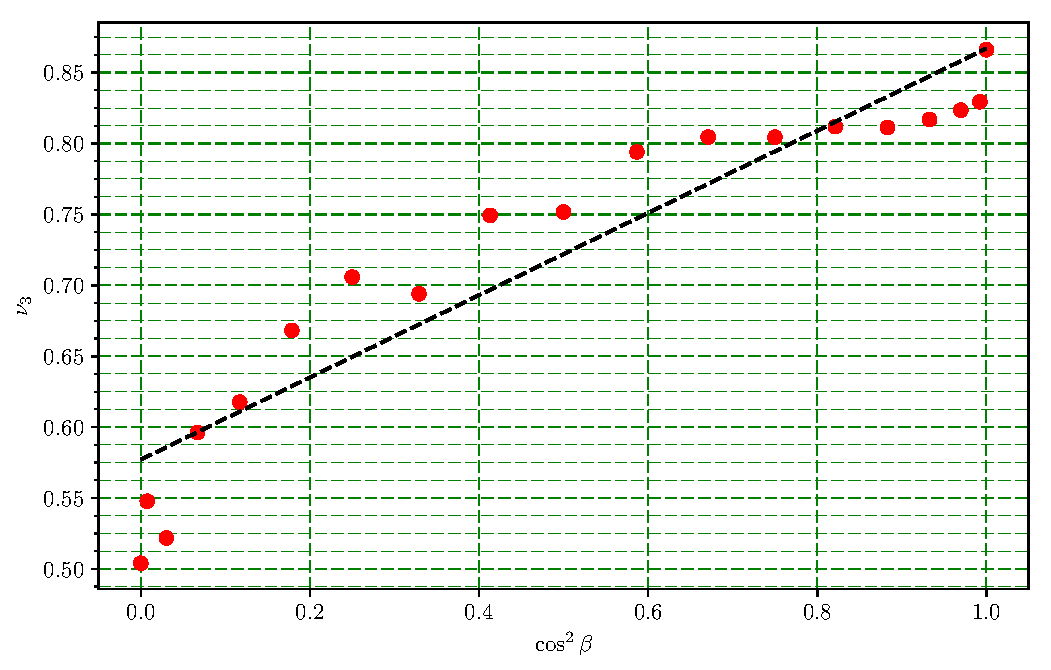
\includegraphics[width = 0.9\lw]{graph}
	\caption{График зависимости $\sin \varphi (\lambda)$}
	\label{fig:graph}
\end{figure}

\item Определим по графику коэффициент наклона и с помощью него найдем шаг решетки:
\[k_+ =  2.00 \pm 0.003~\mkm \]
\[k_- = 1.99 \pm 0.006~\mkm \]
\[d = \pm \dfrac{\lambda}{\sin \varphi} \]
Итого: $d = 2.00 \pm 0.004~\mkm $

\item Для оценки угловой дисперсии решетки определим угловые координаты линий желтой пары во всех видимых порядках спектра, положительных и отрицательных.

\begin{table}[H]
\centering
\caption{Определим угловые координаты линий желтой пары во всех видимых порядках спектра}
\begin{tabular}{|c|c|c|c|c|}
\hline
Цвет     & Порядок & $\varphi$ & $\Delta \varphi,~\text{угл. сек}$   & $D, \text{угл.сек/ангстрем}$  \\ \hline
Желтый 1 & 1       & \ang{163;16;22} & \multirow{2}{*}{250}  & \multirow{2}{*}{11.90}  \\ \cline{1-3}
Желтый 2 & 1       & \ang{163;12;12} &                       &                         \\ \hline
Желтый 1 & -1      & \ang{196;45;9}  & \multirow{2}{*}{-226} & \multirow{2}{*}{-10.76} \\ \cline{1-3}
Желтый 2 & -1      & \ang{196;48;55} &                       &                         \\ \hline
Желтый 1 & 2       & \ang{144;47;50} & \multirow{2}{*}{576}  & \multirow{2}{*}{27.43}  \\ \cline{1-3}
Желтый 2 & 2       & \ang{144;38;14} &                       &                         \\ \hline
Желтый 1 & -2      & \ang{215;14;31} & \multirow{2}{*}{-549} & \multirow{2}{*}{-26.14} \\ \cline{1-3}
Желтый 2 & -2      & \ang{215;23;40} &                       &                         \\ \hline
\end{tabular}
\end{table}

\item Рассчитаем экспериментальную угловую дисперсию для  желтой пары в  спектрах разных порядков по формуле:
\[ D = \dfrac{\Delta \varphi}{\Delta \lambda}, \]
где $\Delta \lambda = 21~\angstrom$.

\item По полученным данным построим график зависимости $D = f(m)$.

\begin{figure}[H]
\centering
	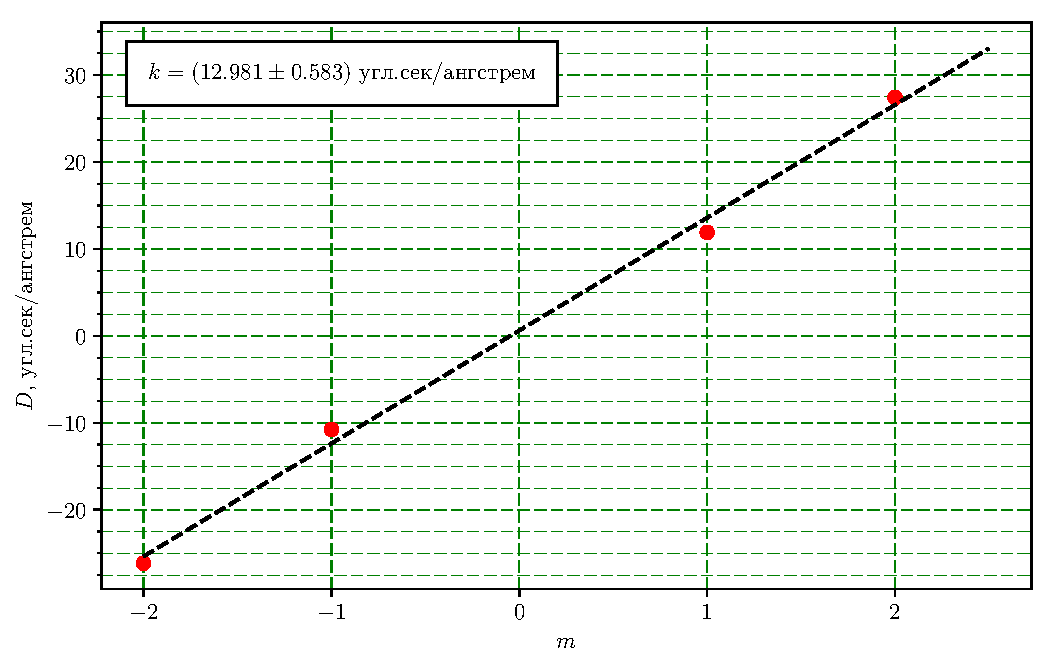
\includegraphics[width = 0.9\lw]{graph1}
	\caption{График зависимости $D = f(m)$}
	\label{fig:graph1}
\end{figure}

\item По графику определяем коэффициент пропорциональности между $D$ и $m$:
\[k_\text{эксп} = (12.98 \pm 0.58)~\text{угл.сек/ангстрем} = (0.63 \pm 0.03)~1/\mkm \]
\[k_\text{теор} \approx \dfrac{1}{d} = (0.5 \pm 0.02)~1/\mkm \]

\item Определим теоретическую разрешающую способность по формуле:
\[R = \dfrac{\lambda}{\delta \lambda} = \dfrac{D\lambda}{\delta \varphi} = 274.8\]
\item Сравнив её с теоретической, рассчитанной по формуле $R = mN$, оценим число эффективно работающих штрихов $N \approx 275$. Тогда размер освещенной части решетки~$\approx 0.55~\mm$.

\item Рассчитаем порядок спектра, при котором фиолетовая линия наложится на желтую. Используя формулу $d \sin \varphi = m \lambda$, получаем
\[ \dfrac{m_\text{ф}}{m_\text{ж}} = \dfrac{\lambda_\text{ж}}{\lambda_\text{ф}} = 1.43 \approx 10/7\]

\end{enumerate}

\section{Вывод}
В ходе эксперимента мы ознакомились с принципами работы гониометра – оптического прибора для точного измерения углов. В результате измерения угловых координат спектральных линий ртути нашли экспериментально шаг решетки $d = 2.00 \pm 0.004~\mkm $, который довольно точно совпадает с приборным значением $d = 2.00~\mkm$.

С помощью измерения угловой полуширины желтого дублета, мы экспериментально нашли угловые дисперсии для разных порядков. И убедились в верности теоретической зависимости $D(m)$ для малых порядков.
\end{document}
